\documentclass[11pt]{beamer}
\usepackage[T1]{fontenc}
\usepackage[activate]{pdfcprot}
\usepackage[ngerman]{babel}
\usepackage[parfill]{parskip}
\usepackage[utf8]{inputenc}
\usepackage{kurier}
\usepackage{amsmath}
\usepackage{amssymb}
\usepackage{xcolor}
\usepackage{epstopdf}
\usepackage{txfonts}
\usepackage{fancyhdr}
\usepackage{graphicx}
\usepackage{prettyref}
\usepackage{hyperref}
\usepackage{eurosym}
\usepackage{setspace}
\usepackage{units}
\usepackage{eso-pic,graphicx}
\usepackage{icomma}

\definecolor{darkblue}{rgb}{0,0,.5}
\hypersetup{pdftex=true, colorlinks=true, breaklinks=false, linkcolor=black, menucolor=black, pagecolor=black, urlcolor=darkblue}



\setlength{\columnsep}{2cm}


\newcommand{\arcsinh}{\mathrm{arcsinh}}
\newcommand{\asinh}{\mathrm{arcsinh}}
\newcommand{\ergebnis}{\textcolor{red}{\mathrm{Ergebnis}}}
\newcommand{\fehlt}{\textcolor{red}{Hier fehlen noch Inhalte.}}
\newcommand{\betanotice}{\textcolor{red}{Diese Aufgaben sind noch nicht in der Übung kontrolliert worden. Es sind lediglich meine Überlegungen und Lösungsansätze zu den Aufgaben. Es können Fehler enthalten sein!!! Das Dokument wird fortwährend aktualisiert und erst wenn das \textcolor{black}{beta} aus dem Dateinamen verschwindet ist es endgültig.}}
\newcommand{\half}{\frac{1}{2}}
\renewcommand{\d}{\, \mathrm d}
\newcommand{\punkte}{\textcolor{white}{xxxxx}}
\newcommand{\p}{\, \partial}
\newcommand{\dd}[1]{\item[#1] \hfill \\}

\renewcommand{\familydefault}{\sfdefault}
\renewcommand\thesection{}
\renewcommand\thesubsection{}
\renewcommand\thesubsubsection{}


\usetheme{Marburg}
\usecolortheme{default}

\useinnertheme{default}
\useoutertheme{default}

\beamertemplatenavigationsymbolsempty
\setbeamertemplate{footline}[frame number]

\title{Galaxien}

\subtitle{Eigenschaften und Klassifikation}

\author{Christoph Hansen}

\institute[FH Aachen - Jülich]{Physikingenieurwesen \\ Fachhochschule Aachen-Jülich}

\date[22.05.14]{22. Mai 2014}

\subject{Eigenschaften und Klassifikation von Galaxien}

\keywords{Galaxien, Eigenschaften, Klassifikation, Hubble}






\begin{document}


%Titelseite

\begin{frame}
\titlepage
\end{frame}


%Inhaltsverzeichnis

\begin{frame}
\tableofcontents
\end{frame}


\section{Überblick über die Klassifikation}

\begin{frame}
\frametitle{Überblick über die Klassifikation}
\framesubtitle{Klassifikation allgemein}

\begin{itemize}
\item Klassifikation hängt von der Beobachtung ab
\end{itemize}
\qquad $\Rightarrow$ Hubble's morphologisches Schema



\begin{itemize}
\item Weitere Möglichkeiten
\begin{enumerate}
\item spektrale Analyse
\item Emissions- und Absorbtiosspektrum
\end{enumerate}
\end{itemize}

\end{frame}


\begin{frame}
\frametitle{Überblick über die Klassifikation}
\framesubtitle{Klassifikation nach Hubble}
\begin{figure}
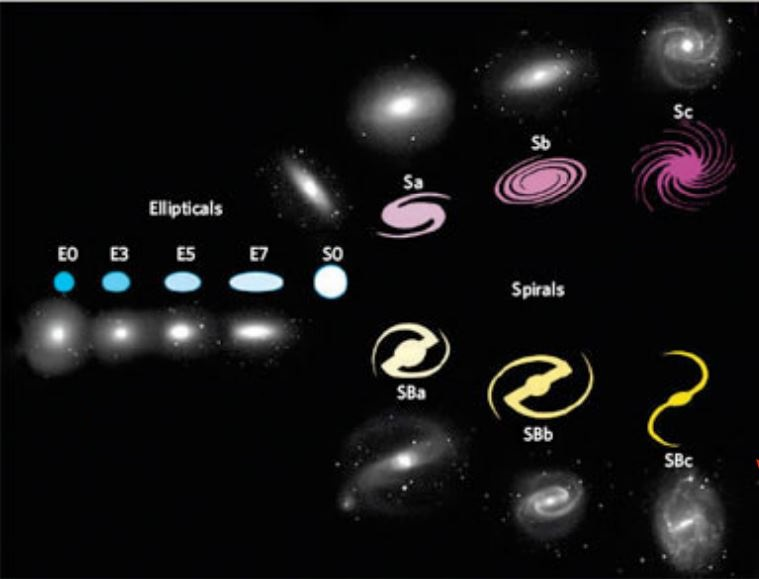
\includegraphics[scale=0.5]{Hubble_Entwicklung.jpg}
\end{figure}
\end{frame}


%\begin{frame}
%\frametitle{Überblick über die Klassifikation}
%\framesubtitle{Klassifikation nach Hubble}

%\begin{itemize}
%\item Elliptische Galaxien
%\item Spiralgalaxien
%\item irreguläre Galaxien
%\end{itemize}

%\end{frame}


\begin{frame}
\frametitle{Überblick über die Klassifikation}
\framesubtitle{Klassifikation nach Hubble}

\begin{itemize}
\item keine Entwicklungssequenz
\item zu geringe Anzahl
\item nur optisch
\item zuerst nur drei Typen
\item nutzlos für Leuchtkraft und Entfernungsmessung
\end{itemize}

\end{frame}

\begin{frame}
\frametitle{Überblick über die Klassifikation}
\framesubtitle{Spektralanalyse}

\begin{figure}
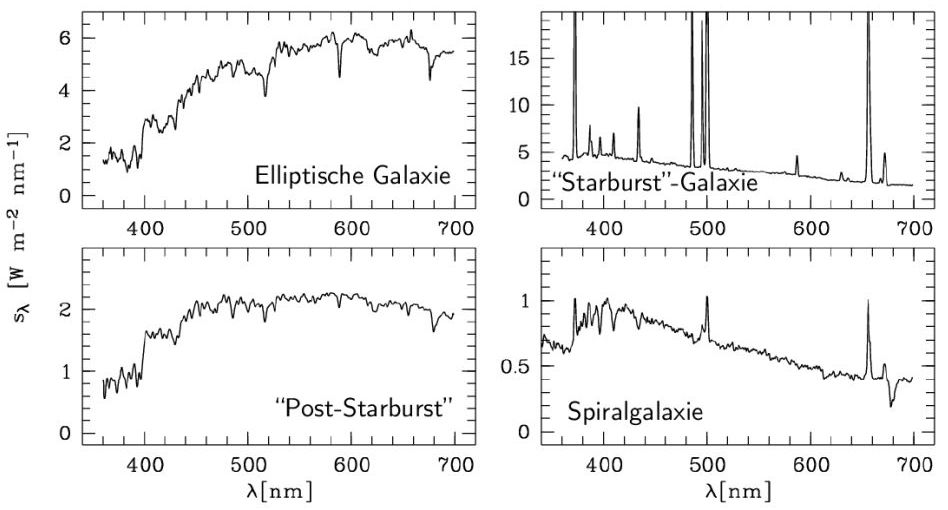
\includegraphics[scale=0.4]{Galaxiespektren.jpg}
\end{figure}

\begin{itemize}
\item Rotverschiebung
\end{itemize}

\end{frame}


\begin{frame}
\frametitle{Überblick über die Klassifikation}
\framesubtitle{Emissions- und Absorbtiosanalyse}


\begin{figure}
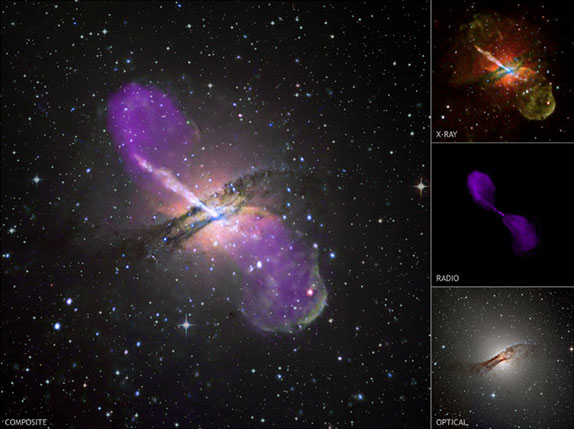
\includegraphics[scale=0.35]{Radiogalaxie.jpg}
\caption{Röntgen, Radio, optisch}
\end{figure}

\begin{itemize}
\item spezifische Emissionslinien für jeden Typ
\end{itemize}


\end{frame}


\section{Galaxientypen}

\begin{frame}
\frametitle{Galaxientypen}
\framesubtitle{Elliptische Galaxien}


\end{frame}





\end{document}